\documentclass{report}
\usepackage{wrapfig}
\usepackage[utf8]{inputenc}
\usepackage{graphicx}
\usepackage{subfigure} 
\usepackage{amsmath, amssymb}
\usepackage[spanish]{babel}
\usepackage{listings}
\usepackage{enumerate}
\usepackage{float}
\usepackage{multirow, array}
\usepackage{vmargin}


\setmargins
{3cm}       % margen izquierdo
{1.5cm}       % margen superior
{15.5cm}      % anchura del texto
{23.42cm}     % altura del texto
{10pt}        % altura de los encabezados
{1cm}         % espacio entre el texto y los encabezados
{0pt}         % altura del pie de página
{2cm}         % espacio entre el texto y el pie de página


\graphicspath{{img/}}

\setcounter{secnumdepth}{0} 
\setcounter{tocdepth}{1} 
\newcounter{ns}
\addtocounter{ns}{1} 

\renewcommand{\figurename}{Figura}
\renewcommand{\tablename}{Tabla}

\begin{document}
	\begin{titlepage}
		\begin{center}
			\vspace*{0in}
			\begin{figure}[htb]
				\begin{center}
					
\includegraphics[width=8cm]{0}
				\end{center}
			\end{figure}
			\rule{80mm}{0.1mm}\\
			\vspace*{0.1in}
			\begin{Large}
				Instituto Tecnológico de Morelia\\
				"José María Morelos y Pavón"\\
			\end{Large}
			\vspace*{0.15in}
			\begin{Large}
				Departamento de Ingeniería Electrónica.\\
			\end{Large}
			\vspace*{0.4in}
			\begin{Large}
				\textbf{PRÁCTICA NO. 2: Polos y ceros encontrados por inspección} \\
				\end{Large}
			\vspace*{0.3in}
			\begin{Large}
				Joani Alonso Hurtado Barrera. 14121123\\
				Daniel Alejandro Marin Magaña. 14121127\\
			\end{Large}
			\vspace*{0.1in}
			\begin{Large}
				Control I\\
				7 Semestre\\
				Grupo A\\
				Fecha de Entrega: 24/10/2017\\
			\end{Large}
		\end{center}		
	\end{titlepage}
%_____________________TERMINA LA PORTADA___________________________________________

\section{Introducción}

El objetivo de esta práctica es el de analizar un circuito RL obteniendo su función de transferencia por dos métodos, inspección y por ecuaciones algebráicas para encontrar los Polos y los Zeros. Obteniendo dicha función se determina su respuesta en el tiempo con la respuesta escalón comprobándola con la función desarrollada en scilab o matlab. Una vez hecho esto se utiliza el software LTSpice para simular el circuito y observer su curva de carga y descarga a su vez que se ve su diagrama de Bode.\\
Con los datos teóricos se lleva el circuito a la práctica armándolo con un generador de frecuencia a la entrada y con el osciloscopio mostrar la curva de carga del inductor para obtener el valor de tao y compararlo con el valor calculado. Posteriormente se hace un barrido de frecuencia tomando captura en cada década de 1Hz a 2MHz, que es la escala máxima del generador. Se muestra una curva similar a la obtenida en el software LTSpice.\\

\section{Metodología}

	Primero que nada obtuvimos nuestra función de transferencia por el método de inspección de la figura 1 como se muestra a continuación:
	
			\begin{figure}[H]
			\begin{center}
				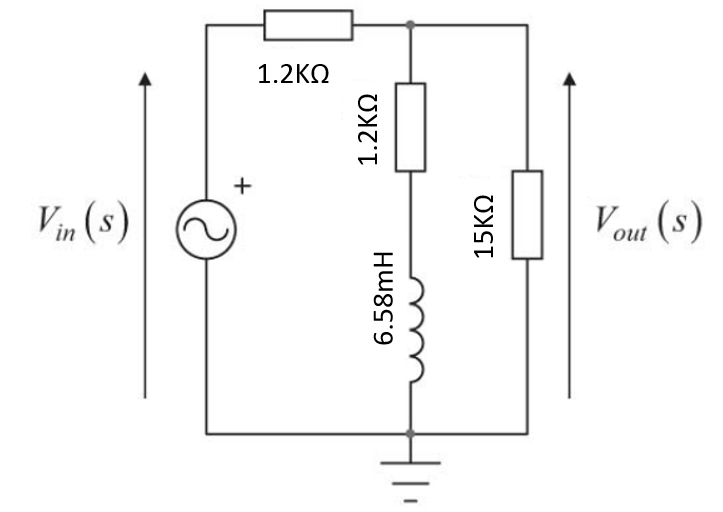
\includegraphics[width=8cm]{6}
				\caption{Circuito RL}
			\end{center}
			\end{figure}
    Sabiendo que:\\
    \begin{equation*}
    Z_L = sL
    \end{equation*}
		
	Para obtener $G_0$ en DC el inductor L se cortocircuita por lo que:
	\[V_{out}(s)=\frac{V_{in}(s)(R_1||R_2)}{R_1+R_2||R_3}\]
	\[\frac{V_{out}(s)}{V_{in}(s)}=\frac{R_2||R_3}{R_1+R_2||R_3}=G_0\]
	Para $W={z1}$ se busca la rama que puede provocar que la salida sea 0:
	\[R_2+sL=0\]
	\[R_2(1+\frac{sL}{R_2})=0\]
	\[1+\frac{sL}{R_2}=0\]
	\[W_{z1}=\frac{R_2}{L}\]
	Para $W_{p1}$ se ponen en corto circuito las fuentes de voltaje y se abren as corriente, sabiendo que $W_{p1}$ tiene que ser $\frac{R_{eq}}{L}$ entonces:
	\[W_{p1}=\frac{R_2+R_1||R_3}{L}\]
	Entonces nuestra función de transferencia es:
	\[H(s)=\frac{R_2||R_3}{R_1+R_2||R_3}*\frac{1+s\frac{L}{R_2}}{1+s\frac{L}{R_2+R_1||R_3}}\]\\
	
	Usando el método algebraico también obtuvimos la misma función de transferencia:
	
	Primero se resuelve la resistencia en Serie de R2 y SL.\\
	
	\begin{equation*}
	R_{es1} = R2 + SL
	\end{equation*}
	
	En seguida se resuelve la resistencia en paralelo con R3 y RES1.\\
	
	\begin{equation*}
	R_{p1} = \frac{R3(R2 + SL)}{R3 + R2 + SL}
	\end{equation*}
	
	Con estas dos impedancias se hace un divisor de voltaje y se obtiene el valor de $V_{out}$.\\
	
	\begin{equation*}
	V_{out}=\frac{V_{in}(\frac{R3(R2 + SL)}{R3 + R2 + SL})}{R1 + \frac{R3(R2 + SL)}{R3 + R2 + SL}}
	\end{equation*}
	
	Como la función de transferencia es $V_{out}/V_{in}$ de la ecuación anterior se simplifica y $V_{in}$ se pasa del otro lado de la igualdad.\\
	
	\begin{equation*}
	\frac{V_{out}}{V_{in}} = \frac{R3(R2 + SL)}{R1R3 + R1R2 + R1SL + R3R2 + R3SL}
	\end{equation*}
	
	LLevándolo a la forma de la ecuación de transferencia general se obtiene lo siguiente:
	
	\begin{equation*}
	\frac{V_{out}}{V_{in}} = \frac{R3R2(1 + \frac{SL}{R2})}{R1(R3 + R2) + R3R2 + R1SL + R3SL}
	\end{equation*}
	
	\begin{equation*}
	\frac{V_{out}}{V_{in}} = \frac{R3R2(1 + \frac{SL}{R2})}{(R1(R3 + R2) + R3R2)(1 + \frac{R1SL + R3SL}{(R1(R3 + R2) + R3R2)})}
	\end{equation*}
	
	\begin{equation*}
	\frac{V_{out}}{V_{in}} = \frac{R3R2(1 + \frac{SL}{R2})}{(R1(R3 + R2) + R3R2)(1 + \frac{SL(R1 + R3)}{(R1R3 + R1R2 + R3R2)})}
	\end{equation*}
	
	Donde:\\
	
	\begin{equation*}
	W_{z1} = R2
	\end{equation*}
	
	y
	
	\begin{equation*}
	W_{p1} = \frac{(R1R3 + R1R2 + R3R2)}{L(R1 + R3)}
	\end{equation*}
	
	Después usando la función creada por nosotros en Scilab también pudimos ver la respuesta de este sistema:  
	Para lograr esto se emplea la ecuación general con el escalon unitario y resolviendo las fracciones parciales:
	
	\begin{equation*}
	\frac{bs + c}{s(sd + a)} = \frac{A}{s} + \frac{B}{s + a}
	\end{equation*}
	
	\begin{equation*}
	A = \frac{c}{a}
	\end{equation*}
	
	\begin{equation*}
	B = b - \frac{cd}{a}
	\end{equation*}
	
	La respuesta en el tiempo es la siguiente:
	
	\begin{equation*}
	H(t) = \frac{c}{a} + (\frac{ba - cd}{ad})(exp^{(\frac{-a}{d})t})
	\end{equation*}
	
	Esta ecuación es implementada en Matlab, los valores de a, b, c y d se identifican en la ecuación de transferencia obtenida anteriormente. Estos valores se deducen sustituyendo los valores R1, R2, R3 y de L con los valores reales, 1.2K$\Omega$, 1.2K$\Omega$, 15K$\Omega$ y 6.58mH, respectivamente,
	
	\begin{lstlisting}[frame=single]
	a = 1;
	b = 2.636217944E-6;
	c = 0.48076923;
	d = 2.847115385E-6;
	t=0:0.01:0.5;
	Y1=(c./a) + (((b*a) - (c*d))./(d*a))*(exp(-(a./d)*t));
	
	plot(t,Y1)
	\end{lstlisting}
	
	\begin{figure}[h]
		\centering
		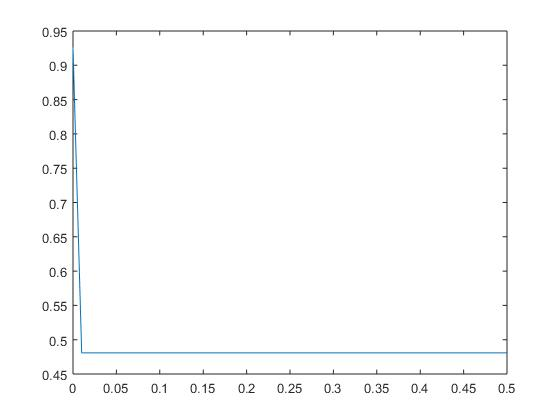
\includegraphics[width=8cm]{graf}
		\caption{Respuesta en el tiempo con MATlab}\label{figura 1}
	\end{figure}

\newpage

	y finalmente revisamos la respuesta de la figura 1 usando LTI spice:
	
	\begin{lstlisting}[frame=single]
	;Circuito practica 2
	Vin 1 0  pulse (0V,5V,0s,1ns,1ns,1ms,2ms) ;AC 1
	R1 1 2 1.2K
	R2 2 3 1.2k
	R3 2 0 15K
	L1 3 0 6.58mH
	;.tran 100us 10ms 1us
	;.ac dec 10 10Hz 500KHz
	.tran 1us 2ms
	.end
	\end{lstlisting}
	
	\begin{figure}[h]
		\centering
		\includegraphics[width=15cm]{captura1}
		\caption{Señales de salida, V(3) y entrada, V(1)}\label{figura 2}
	\end{figure}

\begin{lstlisting}[frame=single]
;Circuito practica 2
Vin 1 0   AC 1 ;pulse (0V,5V,0s,1ns,1ns,1ms,2ms)
R1 1 2 1.2K
R2 2 3 1.2k
R3 2 0 15K
L1 3 0 6.58mH
;.tran 100us 10ms 1us
.ac dec 10 1Hz 2000KHz
;.tran 1us 2ms
.end
\end{lstlisting}

\begin{figure}[h]
	\centering
	\includegraphics[width=15cm]{captura3}
	\caption{Diagrama de bode}\label{figura 3}
\end{figure}
	
\section{Resultados}

	Construyendo el circuito de la figura 1 físicamente se hizo un barrido de frecuencias desde $1Hz$ hasta $2MHz$ debido a que el generador es la máxima frecuencia que alcanza.
	
	de donde podemos calcular $\tau$ de la siguiente manera:
	\[\tau=\frac{L}{R_{eq}}=\frac{6.58mH}{R_2+R_1||R_3}=\frac{6.58mH}{2.31K\Omega}=2.83mS\]
	
\begin{table}[H]
	\centering
	\caption{Valores obtenidos del barrido de frecuencia}
	\begin{tabular}{r|r|r|r}
		\multicolumn{1}{l}{Frecuencia} & \multicolumn{1}{l}{Vmax} & \multicolumn{1}{l}{Frecuencia} & \multicolumn{1}{l}{Vmax} \\
		1     & 0.44  & 2000  & 1.12 \\
		2     & 0.688 & 3000  & 1.12 \\
		3     & 0.832 & 4000  & 1.12 \\
		4     & 0.912 & 5000  & 1.12 \\
		5     & 1     & 6000  & 1.14 \\
		6     & 1.08  & 7000  & 1.14 \\
		7     & 1.08  & 8000  & 1.14 \\
		8     & 1.08  & 9000  & 1.16 \\
		9     & 1.12  & 10000 & 1.16 \\
		10    & 1.12  & 20000 & 1.28 \\
		20    & 1.12  & 30000 & 1.44 \\
		30    & 1.12  & 40000 & 1.56 \\
		40    & 1.12  & 50000 & 1.64 \\
		50    & 1.12  & 60000 & 1.76 \\
		60    & 1.12  & 70000 & 1.82 \\
		70    & 1.12  & 80000 & 1.9 \\
		80    & 1.12  & 90000 & 1.94 \\
		90    & 1.12  & 100000 & 1.98 \\
		100   & 1.12  & 200000 & 2.14 \\
		200   & 1.12  & 300000 & 2.06 \\
		300   & 1.12  & 400000 & 1.98 \\
		400   & 1.12  & 500000 & 1.8 \\
		500   & 1.12  & 600000 & 1.68 \\
		600   & 1.12  & 700000 & 1.6 \\
		700   & 1.12  & 800000 & 1.52 \\
		800   & 1.12  & 900000 & 1.42 \\
		900   & 1.12  & 1000000 & 1.34 \\
		1000  & 1.12  & 2000000 & 1.22 \\
	\end{tabular}%
	\label{tab:addlabel}%
\end{table}%
	
	\begin{figure}[H]
		\begin{center}
			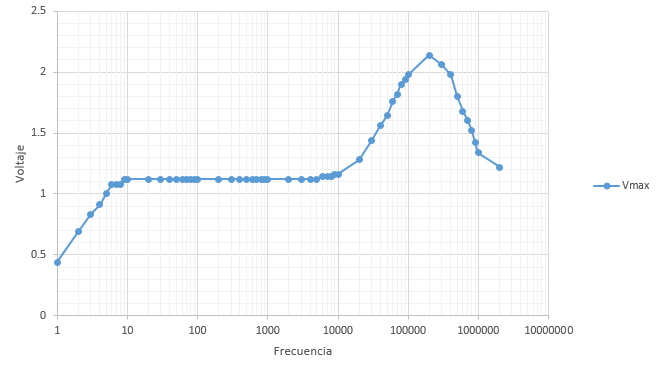
\includegraphics[width=11cm]{3}
			\caption{comportamiento del voltaje $V_{max}$ con respecto al incremento de la frecuencia}
		\end{center}
	\end{figure}

	y de acuerdo a la figura 3 se pudo medir un primer $\tau$ que pasa al 63\% del voltaje máximo, donde nuestro $V_{max}=4.3V$ y a $V=2.709V$ que es el 63\% de nuestro $V_{max}$ nuestro $\tau=132nS$
	
	\begin{figure}[H]
	\begin{minipage}[b]{0.5\linewidth} %Una minipágina que cubre la mitad de la página
		\centering
		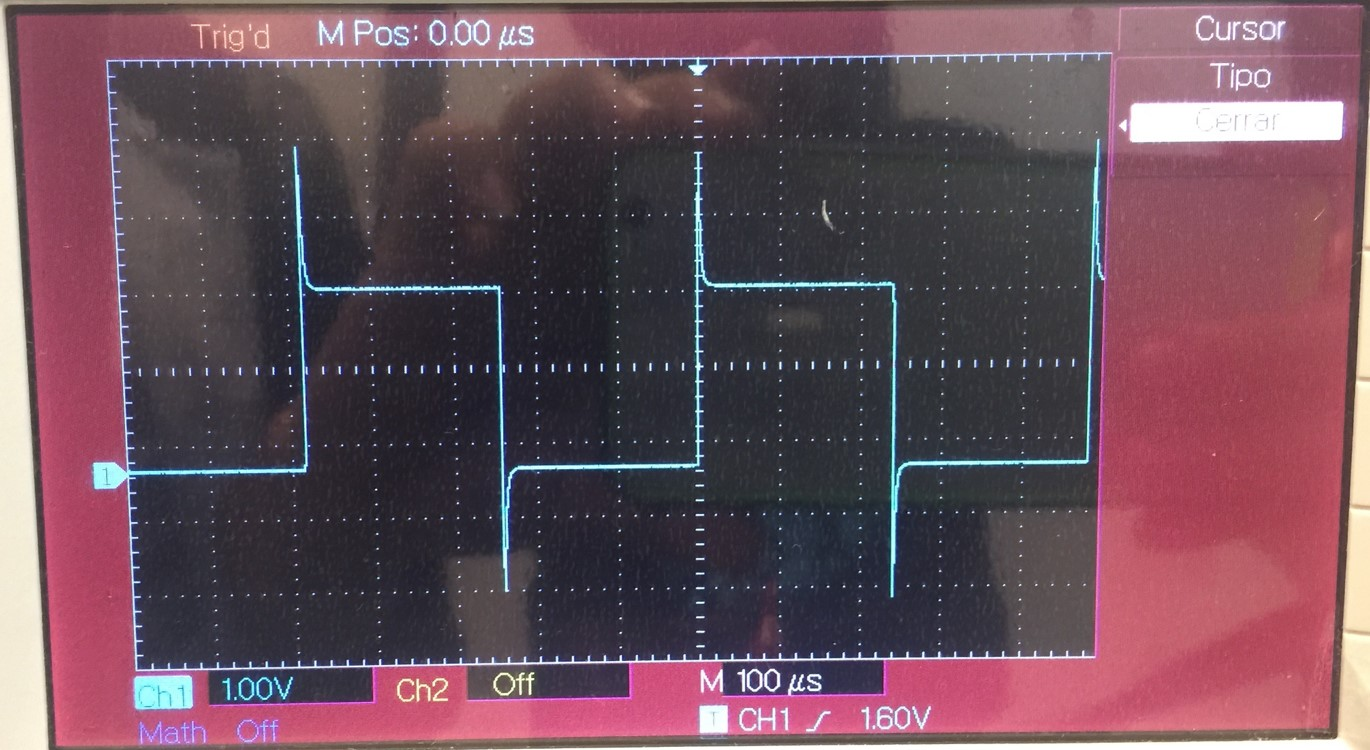
\includegraphics[width=6cm]{5}
		\caption{Señal de la resistencia de carga $R_3$}\label{fig3}
	\end{minipage}
	\hspace{0.5cm} % Si queremos tener un poco de espacio entre las dos figuras
	\begin{minipage}[b]{0.5\linewidth}
		\centering
		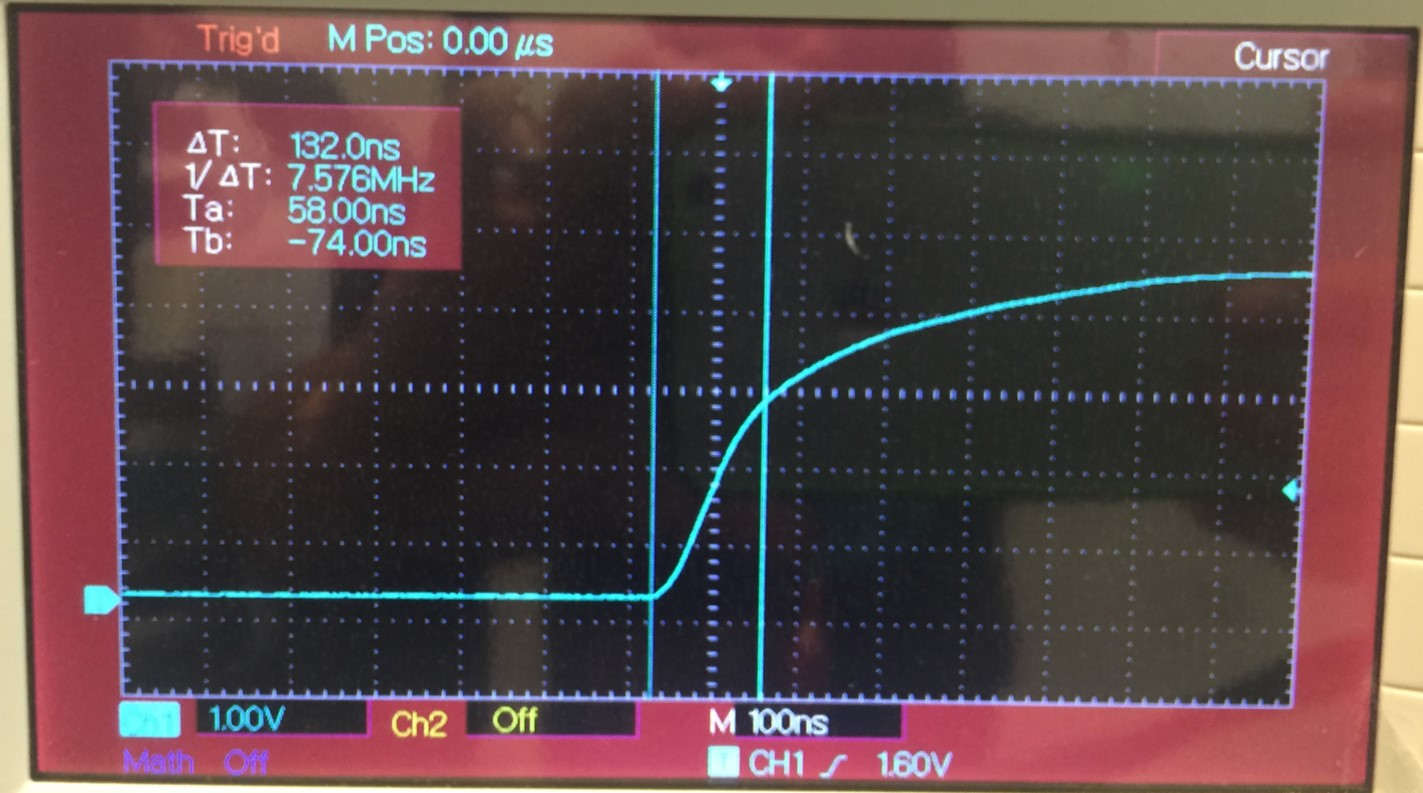
\includegraphics[width=6cm]{4}
		\caption{Primer $\tau$}\label{fig4}
	\end{minipage}
	\end{figure}
	
\section{Conclusiones}
	\subsection{Joani Alonso Hurtado Barrera:}
	En esta práctica y durante la realización de la misma aprendimos como es que es mucho más fácil y rápido obtener la función de transferencia de un circuito sencillo como lo es el que nos toco analizar que se trata de un circuito RL y así mismo poder visualizar más rápido lo que es la ganancia del circuito y sus raíces, así mismo aprendimos como esta función de transferencia nos permite conocer bastante a cerca del circuito en cuestión y finalmente ahora sabemos que existen varias herramientas que nos permiten comprobar y apoyar nuestros resultado, también simular y ver un comportamiento aproximado a la realidad, el único inconveniente que tuvimos en esta practica fue que el $\tau$ no fue el que esperábamos, pero hay muchos factores en el diseño del inductor que afecta esto. 
	
	\subsection{Daniel Alejandro Marín Magaña:}
	Analizar circuitos complejos en donde no sólo haya elementos resistivos, si no también inductivos puede llegar a ser sencillo si se utiliza el método adecuado para determinar su ecuación de transferencia. Con esta ecuación se puede obtener mucha información del circuito, por ejemplo la locación de los polos y zeros, que nos determinan en que punto el circuito es estable.\\
	El comportamiento del circuito fue analizado teóricamente, en simulación y prácticamente. Teóricamente se aprendió a determinar la ecuación de transferencia con dos métodos, inspección, que consta de observar el circuito y a simple vista obtener sus parámetros, y por ecuaciones algebráicas, que es analizar el circuito con ley de Ohm. En las simulaciones se usaron los software MATlab y LTSpice para graficar dicha ecuación y observar su comportamiento, con LTSpice se observó también el diagrama de Bode, y finalmente en la práctica fue armar el circuito y hacer un barrido de frecuencia y graficar los valores de voltaje obtenidos de voltaje máximo, sin embargo se presentó un error en la medición de $\tau$, ya que se calculó pero en el momento de medirlo en el osciloscopio no se obtuvo el valor esperado, existen varios factores que pudieron afectar a esto, la frecuencia, el tipo de inductor, etc.


\end{document}
